\documentclass[solution,addpoints,12pt]{exam}
\usepackage{amsmath}
\usepackage{amsthm}
\usepackage{amssymb}
\usepackage{tikz}
\usepackage{animate}
\usepackage{hyperref}
\usepackage{comment}
\usepackage{caption}

\newtheorem{theorem}{Theorem}
\newtheorem{lemma}[theorem]{Lemma}

\newenvironment{Solution}{\begin{EnvFullwidth}\begin{solution}}{\end{solution}\end{EnvFullwidth}}

\printanswers
%\unframedsolutions
\pagestyle{headandfoot}

%%%%%%%%%%%%%%%%%%%%%%%%%%%%%%%%%%%%%%%%%%%%%%%%%%%%%%
%%%%%%%%%%%%%%%%%%% INSTRUCTIONS %%%%%%%%%%%%%%%%%%%%%
% * Fill in your name and roll number below

% * Answer in place (after each question)

% * Use \begin{solution} and \end{solution} to typeset
%   your answers.
%%%%%%%%%%%%%%%%%%%%%%%%%%%%%%%%%%%%%%%%%%%%%%%%%%%%%%
%%%%%%%%%%%%%%%%%%%%%%%%%%%%%%%%%%%%%%%%%%%%%%%%%%%%%%

% Fill in the details below
\def\studentName{\textbf{Bikash Gogoi}}
\def\studentRoll{\textbf{CS14B039}}

\firstpageheader{CS 7015 - Deep Learning - Assignment 1}{}{\studentName, \studentRoll}
\firstpageheadrule

\newcommand{\brac}[1]{\left[ #1 \right]}
\newcommand{\curly}[1]{\left\{ #1 \right\}}
\newcommand{\paren}[1]{\left( #1 \right)}
\newcommand{\card}[1]{\left\lvert #1 \right\rvert}

\begin{document}

Instructions:
\begin{itemize}
    \itemsep0em
    \item This assignment is meant to help you grok certain concepts we will use in the course. Please don't copy solutions from any sources.
    \item Avoid verbosity.
    \item Questions marked with * are relatively difficult. Don't be discouraged if you cannot solve them right away!
    \item The assignment needs to be written in latex using the attached tex file. The solution for each question should be written in the solution block in space already provided in the tex file. \textbf{Handwritten assignments will not be accepted.}
\end{itemize}

\noindent\rule{\textwidth}{1pt}

\begin{questions}



\question \textbf{Partial Derivatives}
          \newline
          \begin{parts}
   
            \part Consider the following computation ,
                  \begin{center}
                    \tikzstyle{neuron}=[circle,draw=blue!50,fill=blue!20,thick,minimum size=10mm]
                    \tikzstyle{input}=[circle,draw=black!50,fill=black!20,thick,minimum size=6mm]
                    \begin{tikzpicture}
                        \node [neuron] (neuron0) at (1,6)  {$\frac{1 + tanh(\frac{wx+b}{2})}{2}$} ;
                        \node (input1) at (-1,6)  {$x$};
                        \node (input0) at (-1,5)  {$1$};
                        \node (output0) at (3,6)  {$f(x)$};
                        \node (formula) at (0,4) {where $f(x) = \frac{1 + tanh(\frac{wx+b}{2})}{2}$ and by definiton : $tanh(z) = \frac{e^{z} - e^{-z}}{e^{z} + e^{-z}} $};
                        \draw [->] (input0) -- (neuron0);
                        \draw [->] (input1) -- (neuron0);
                        \draw [->] (neuron0) -- (output0);
                    \end{tikzpicture}
                  \end{center}
                  The value $L$ is given by, 
                  \[ 
                     L = \frac{1}{2} (y - f(x))^2
                  \]
                  Here, $x$ and $y$ are constants and $w$ and $b$ are parameters that can be modified.
                  In other words, $L$ is a function of $w$ and $b$.

                  Derive the partial derivatives, $\frac{\partial L}{\partial w}$ and $\frac{\partial L}{\partial b}$.
   
              \begin{solution}
              	\begin{align*}
              	 \frac{\partial L}{\partial f(x)} &= f(x) - y\\
              	 \frac{\partial f(x)}{\partial tanh(\frac{wx+b}{2})} &= \frac{1}{2}\\
              	 \frac{\partial tanh(\frac{wx+b}{2})}{\partial (\frac{wx+b}{2})} &= 1 - tanh^2(\frac{wx+b}{2})\\
              	 \frac{\partial (\frac{wx+b}{2})}{\partial w} &= \frac{x}{2}\\
              	 \frac{\partial (\frac{wx+b}{2})}{\partial b} &= \frac{1}{2}
              	 \end{align*}
              	 \begin{align*}        	 
              	 \frac{\partial L}{\partial w} &= \frac{\partial L}{\partial f(x)} \times \frac{\partial f(x)}{\partial tanh(\frac{wx+b}{2})} \times \frac{\partial tanh(\frac{wx+b}{2})}{\partial (\frac{wx+b}{2})} \times \frac{\partial (\frac{wx+b}{2})}{\partial w}\\
              	 &= (f(x) - y) \times \frac{1}{2} \times (1 - tanh^2(\frac{wx+b}{2})) \times \frac{x}{2}
				\end{align*}
				\begin{align*}              	 
              	 \frac{\partial L}{\partial b} &= \frac{\partial L}{\partial f(x)} \times \frac{\partial f(x)}{\partial tanh(\frac{wx+b}{2})} \times \frac{\partial tanh(\frac{wx+b}{2})}{\partial (\frac{wx+b}{2})} \times \frac{\partial (\frac{wx+b}{2})}{\partial b}\\
              	 &= (f(x) - y) \times \frac{1}{2} \times (1 - tanh^2(\frac{wx+b}{2})) \times \frac{1}{2}
              	\end{align*}
              \end{solution}
  
            \part Consider the evaluation of $E$ as given below,
                  \[
                    E = g(x,y,z) = \sigma(c(ax + by) + dz)
                  \]
                  Here $x,y,z$ are inputs (constants) and $a,b,c,d$ are parameters (variables). $\sigma$ is the logistic sigmoid function defined as:
                  \[
                    \sigma(x) = \frac{1}{1 + e^{-x}}    
                  \]

                  Note that here $E$ is a function of $a,b,c,d$.


                  Compute the partial derivatives of $E$ with respect to the parameters $a$, $b$ and $d$ i.e. $\frac{\partial E}{\partial a}$, $\frac{\partial E}{\partial b}$ and $\frac{\partial E}{\partial d}$.
             
              
              \begin{solution}
					Let $p = c(ax+by) + dz$              	
              	\begin{align*}
              		\frac{\partial E}{\partial p} &= \sigma (p)(1 - \sigma (p))\\
              		\frac{\partial p}{\partial a} &= cx\\
              		\frac{\partial p}{\partial b} &= cy\\
              		\frac{\partial p}{\partial d} &= z
              	\end{align*}
              	\begin{align*}
              		\frac{\partial E}{\partial a} &= \frac{\partial E}{\partial p} \times \frac{\partial p}{\partial a}\\
              										&= \sigma (p)(1 - \sigma (p)) \times cx
              	\end{align*}
              	\begin{align*}
              		\frac{\partial E}{\partial b} &= \frac{\partial E}{\partial p} \times \frac{\partial p}{\partial b}\\
              										&= \sigma (p)(1 - \sigma (p)) \times cy
              	\end{align*}
              	\begin{align*}
              		\frac{\partial E}{\partial d} &= \frac{\partial E}{\partial p} \times \frac{\partial p}{\partial d}\\
              										&= \sigma (p)(1 - \sigma (p)) \times z
              	\end{align*}
              \end{solution}


          \end{parts}        

\question \textbf{Erroneous Estimates}
\newline
The first order derivative of a real valued function $f$ is defined by the following limit (if it exists),
          \begin{equation} \label{eq:deriv_definition}
            \frac{df(x)}{dx} = \lim_{h \to 0} \frac{f(x + h) - f(x)}{h}
          \end{equation}
          On observing the above definition we see that the derivative of a function is the ratio of
          change in the function value to the change in the function input, 
          when we change the input by a small quantity (infinitesimally small).

          Consider the function $f(x) = x^2 - 2x + 1$. 
        \begin{parts}
        
        \part Using the limit definition of derivative, show that the derivative of $f(x)$ is $\frac{df(x)}{dx} = 2x - 2$.
        \begin{solution}
        	\begin{align*}
        		f(x) &= x^2 - 2x + 1\\
        		\frac{df(x)}{dx} &= \lim_{h \to 0} \frac{f(x + h) - f(x)}{h}\\
        						&= \lim_{h \to 0} \frac{\{(x+h)^2 - 2(x+h) + 1\} - (x^2 - 2x + 1)}{h}\\
        						&= \lim_{h \to 0} \frac{2xh + h^2 - 2h}{h}\\
        						&= \lim_{h \to 0} 2x - 2 + h\\
        						&= 2x - 2
        	\end{align*}
        \end{solution}
        
        \part The function evaluates to $0$ at $1$ i.e. $f(1) = 0$. 
        
          Say we wanted to estimate the value of $f(1.01)$ and $f(1.5)$ without using the definition of $f(x)$. We could think of using the definition of derivative to ``extrapolate'' the value of $f(1)$ to obtain $f(1.01)$ and $f(1.5)$.

          A first degree approximation based on \ref{eq:deriv_definition} would be the following.
          \begin{equation}
            f(x+h) \approx f(x) + h \frac{df(x)}{dx}
          \end{equation}

        Estimate $f(1.01)$ and $f(1.5)$ using the above formula.
                  \begin{solution}
                  	\begin{align*}
                  		f(1.01) = f(1 + 0.01) &\approx f(1) + 0.01 \times \left[\frac{df(x)}{dx}\right]_{x=1}\\
                  							&= 0 + 0.01 \times \left[(2x - 2)\right]_{x=1}\\
                  							&= 0
                  	\end{align*}
                  	\begin{align*}
                  		f(1.5) = f(1 + 0.5) &\approx f(1) + 0.5 \times \left[\frac{df(x)}{dx}\right]_{x=1}\\
                  							&= 0 + 0.5 \times \left[(2x - 2)\right]_{x=1}\\
                  							&= 0
                  	\end{align*}
                  \end{solution}
                  
            \part Compare it to the actual value of $f(1.01) = 0.0001$, and $f(1.5) = 0.25$.
                  \begin{solution}\\
                  	Error in $f(1.01) = 0.0001$\\
                  	Error in $f(1.5) = 0.25$
                  \end{solution}
            \part Explain the discrepancy from the actual value. Why does it increase/decrease when we move
                  further away from $1$?
                  \begin{solution}
                  		Since at point $x=1$, $f(x)$ achieves local minima, so the value of $f(x)$ increases as we move away from it.
                  \end{solution}
            \part Can we get a better estimate of $f(1.01)$ and $f(1.5)$ by ``correcting'' our estimate from part $(a)$? Can you suggest a way of doing this?
                  \begin{solution}
                  	Yes we can do better. Instead of using only first order terms of the taylor series, we can used second order terms as well.\\
                  	So, $f(x + h) \approx f(x) + h \times \frac{df(x)}{dx} + \frac{h^2}{2!} \times \frac{d^2f(x)}{dx^2}$
                  	
                  \end{solution}
          \end{parts}
          


\question \textbf{Differentiation w.r.t. Vectors and matrices}
          \newline
          Consider vectors $\boldsymbol{u, x} \in \mathbb{R}^d$, and matrix $\boldsymbol{A} \in \mathbb{R}^{n \times n}$.
          \newline
          The gradient of a scalar function $f$ w.r.t. a vector $\boldsymbol{x}$ is a vector by itself, given by
          \[
            \nabla_{\mathbf{x}} f = \left( \frac{\partial f}{\partial x_1}, \frac{\partial f}{\partial x_2}, \dots, 
                         \frac{\partial f}{\partial x_n} 
                       \right)
          \]
          Gradient of a scalar function w.r.t a matrix is a matrix. 
          \[
            \nabla_{\mathbf{A}} f = \begin{bmatrix} 
                \frac{\partial f}{\partial A_{11}} & \frac{\partial f}{\partial A_{12}} & \dots & \frac{\partial f}{\partial A_{1n}}\\
                \frac{\partial f}{\partial A_{21}} & \frac{\partial f}{\partial A_{22}} & \dots & \frac{\partial f}{\partial A_{2n}}\\
                \vdots & \vdots & \ddots & \vdots\\
                \frac{\partial f}{\partial A_{n1}} & \frac{\partial f}{\partial A_{n2}} & \dots & \frac{\partial f}{\partial A_{nn}}\\
                       \end{bmatrix}
          \]
          Gradient of the gradient of a function w.r.t. a vector is a matrix. It is referred to as Hessian. 
          \[
            \mathbf{H}_{\mathbf{x}} f = \nabla_{\mathbf{x}}^2 f = \begin{bmatrix} 
                \frac{\partial^2 f}{\partial^2 x_1} & \frac{\partial^2 f}{\partial x_1 \partial x_2} & \dots & \frac{\partial^2 f}{\partial x_1 \partial x_n}\\
                \frac{\partial^2 f}{\partial x_2  \partial x_1} & \frac{\partial^2 f}{\partial^2 x_2} & \dots & \frac{\partial^2 f}{\partial x_2 \partial x_n}\\
                \vdots & \vdots & \ddots & \vdots\\
                \frac{\partial^2 f}{\partial x_n  \partial x_1} & \frac{\partial^2 f}{\partial x_n \partial x_2} & \dots & \frac{\partial^2 f}{\partial^2 x_n}\\
                       \end{bmatrix}
          \]
          \newline
          \begin{parts}
              
          \part Derive the expressions for the following gradients.
          \begin{enumerate}
              \item $\nabla_{\mathbf{x}} \boldsymbol{u^T x}$
             \item $\nabla_{\mathbf{x}} \boldsymbol{x^T x}$ 
             \item $\nabla_{\mathbf{x}} \boldsymbol{x^T A x} $
             \item $\nabla_{\mathbf{A}} \boldsymbol{x^T A x}$ 
             \item $\nabla^2_{\mathbf{x}} \boldsymbol{x^T A x}$
          \end{enumerate}
          (Aside: Compare your results with derivatives for the scalar equivalents
          of the above expressions $ax$ and $x^2$.)

          The gradient of a scalar $f$ w.r.t. a matrix $\boldsymbol{X}$, is a matrix whose $(i,j)$ component is $\frac{\partial f}{\partial X_{ij}}$, where $X_{ij}$ is the $(i,j)$ component of the matrix $\boldsymbol{X}$.)
          \begin{solution}
          	\begin{enumerate}
          		\item
          			\begin{align*}
          				\nabla_{\mathbf{x}} \boldsymbol{u^T x} &= \nabla_{\mathbf{x}} f\\
          				f &= \sum_{i=1}^{n} u_ix_i\\
          				\frac{\partial f}{\partial x_i} &= u_i\\
          				\nabla_{\mathbf{x}} f &= \left(\frac{\partial f}{\partial x_1}, \frac{\partial f}{\partial x_2}, \dots, \frac{\partial f}{\partial x_n}\right)\\
          						&= \left(u_1, u_2, \dots, u_n\right)\\
          						&= \boldsymbol{u^T}
          			\end{align*}
          		
          		\item
          			\begin{align*}
          				\nabla_{\mathbf{x}} \boldsymbol{x^T x} &= \nabla_{\mathbf{x}} f\\
          				f &= \sum_{i=1}^{n} x_i^2\\
          				\frac{\partial f}{\partial x_i} &= 2x_i\\
          				\nabla_{\mathbf{x}} f &= \left(\frac{\partial f}{\partial x_1}, \frac{\partial f}{\partial x_2}, \dots, \frac{\partial f}{\partial x_n}\right)\\
          						&= \left(2x_1, 2x_2, \dots, 2x_n\right)\\
          						&= 2\boldsymbol{x^T}
          			\end{align*}
          			
          		\item
          			\begin{align*}
          				\nabla_{\mathbf{x}} \boldsymbol{x^TAx} &= \nabla_{\mathbf{x}} f\\
						f &= \boldsymbol{x^TAx}\\          				
          				  &= \sum_{i=1}^{n} x_i \sum_{j=1}^{n} x_j a_{ij}\\
          					&= \sum_{i=1}^{n} \sum_{j=1}^{n} x_i x_j a_{ij}
          			\end{align*}
          			\begin{align*}
          				\frac{\partial f}{\partial x_k} &= \sum_{i \neq k} a_{ik} x_i + \sum_{j \neq k} a_{kj} x_j + 2a_{kk}x_k\\
          				&= \sum_{i=1}^{n} a_{ik}x_i + \sum_{j=1}^{n} a_{kj}x_j\\
          				&= \boldsymbol{x^TA_k} + \boldsymbol{x^TA_k^T}\\
          				&= \boldsymbol{x^T} \left(\boldsymbol{A_k} + \boldsymbol{A^T_k} \right)\\
          				&= \boldsymbol{x^T} \left(\boldsymbol{A}+ \boldsymbol{A^T} \right)_k
          			\end{align*}
          			\begin{align*}
          				\nabla_{\mathbf{x}} f &= \left(\boldsymbol{x^T} \left(\boldsymbol{A} + \boldsymbol{A^T}\right)_1, \boldsymbol{x^T} \left(\boldsymbol{A} + \boldsymbol{A^T}\right)_2, \dots, \boldsymbol{x^T} \left(\boldsymbol{A} + \boldsymbol{A^T}\right)_n \right)\\
          				&= \boldsymbol{x^T} \left(\boldsymbol{A} + \boldsymbol{A^T} \right)
          			\end{align*}
          			
          		\item
          			\begin{align*}
          				\nabla_{\mathbf{A}} \boldsymbol{x^TAx} &= \nabla_{\mathbf{A}} f\\
          				f &= \sum_{i=1}^{n} \sum_{j=1}^{n} x_ix_ja_{ij}\\
          				\frac{\partial f}{a_{ij}} &= x_i x_j\\
          			\end{align*}
\[          				\nabla_{\mathbf{A}} f = 
					\begin{bmatrix}  									
							x_1^2 & x_1x_2 &\ \dots & x_1x_n\\
          					x_2x_1 & x_2^2 & \dots & x_2x_n\\
          					\vdots & \vdots & \ddots & \vdots\\
          					x_nx_1 & x_nx_2 & \dots & x_nx_n
          			\end{bmatrix} = \boldsymbol{xx^T}
\]

				\item
					\begin{align*}
						\nabla_{\mathbf{x}}^2 \boldsymbol{x^TAx} &= \nabla_{\mathbf{x}} f\\
						f &= \sum_{i=1}^{n} \sum_{j=1}^{n} x_ix_ja_{ij}\\
						\frac{\partial f}{\partial x_t} &= \sum_{i \neq t} a_{it}x_i + \sum_{j \neq t} a_{tj} + 2a_{tt}x_t\\
						\frac{\partial f}{\partial x_s \partial x_t} &= \left\{
    						\begin{array}{@{} l c @{}}
      							a_{st} + a_{ts} + 0 & \text{if $s \neq t$} \\
      							0 + 0 + 2a_{tt} & \text{if $s = t$}
    						\end{array}\right.\\
    						&= \left(\boldsymbol{A} + \boldsymbol{A^T}\right)_{st}\\
    						\therefore \nabla_{\mathbf{x}}^2 \boldsymbol{x^TAx} &= \boldsymbol{A} + \boldsymbol{A^T}
					\end{align*}
          	\end{enumerate}
          \end{solution}
        
          \part Use the equations obtained in the previous part to get the Linear regression solution that you studied in ML or PR. Suppose $X$ as input example-feature matrix, $Y$ as given outputs and $\mathbf{w}$ as weight vector.
          \begin{solution}
          		\begin{align*}
          			L &= (Y - \hat{Y})^T(Y - \hat{Y})\\
						&= (Y - X\mathbf{w})^T(Y - X\mathbf{w})\\
						&= (Y^T - \mathbf{w}^TX^T)(Y - X\mathbf{w})\\
						&= (Y^TY - Y^TX\mathbf{w} - \mathbf{w}^TX^TY + \mathbf{w}^TX^TX\mathbf{w}\\
					\frac{\partial L}{\mathbf{w}} &= -Y^TX - Y^TX + \mathbf{w}^TX^TX + \mathbf{w}^TX^TX = 0\\
						&\implies \mathbf{w}^TX^TX = Y^TX\\
						&\implies \mathbf{w}^T = Y^TX(X^TX)^{-1}\\
						&\implies \mathbf{w} = (X^TX)^{-1}X^TY
          		\end{align*}
          \end{solution}

          \part By now you must have the intuition. Gradient w.r.t. a 1 dimensional array was 1 dimensional. Gradient w.r.t. a 2-dimensional array was 2 dimensional. Higher order arrays are referred to as tensors. Let T be a 3 dimensional tensor. Write the expression of $\nabla_{\mathbf{T}} f$. You can use gradients w.r.t. a vector or a matrix in the expression. 
          
          \begin{solution}
          \end{solution}

          \end{parts}

\question \textbf{Ordered Derivatives}
          \newline
          An ordered network is a network where the state variables can be computed 
          one at a time in a specified order.

          Answer the following questions regarding such a network.
          \begin{parts}
            \part Given the ordered network below, give a formula for calculating the ordered derivative $\frac{\partial y_4}{\partial y_1}$ in terms of partial derivatives w.r.t. $y_1$ and $y_2$ where $y_1$, $y_2$ and $y_3$ are the outputs of nodes 1, 2 and 3 respectively.
                   \begin{center}
                    \tikzstyle{neuron}=[circle,draw=blue!50,fill=blue!20,thick,minimum size=10mm]
                    \tikzstyle{input}=[circle,draw=black!50,fill=black!20,thick,minimum size=6mm]
                    \begin{tikzpicture}
                        \node [neuron] (neuron0) at (0,2)  {$1$} ;
                        \node [neuron] (neuron1) at (3,4) {$2$} ;
                        \node [neuron] (neuron2) at (3,0)  {$3$} ;
                        \node [neuron] (neuron3) at (6,2)  {$4$} ;
                        \node  (output1) at (1,2)  {$y_1$} ;
                        \node  (output2) at (4,4)  {$y_2$} ;
                        \node  (output3) at (4,0)  {$y_3$} ;
                        \node  (output3) at (7,2.3)  {$y_4$} ;
                        \draw [->] (neuron0) -- (neuron2) ;
                        \draw [->] (neuron0) -- (neuron1) ;
                        \draw [->] (neuron1) -- (neuron2) ;
                        \draw [->] (neuron1) -- (neuron3) ;
                        \draw [->] (neuron2) -- (neuron3) ;
                    \end{tikzpicture}
                    \label{fig:ordered-network}
                  \end{center}
                  \begin{solution}
                  		\begin{align*}
                  			& y_4 = f(y_2, y_3)\\
                  			& y_3 = f(y_1, y_2)\\
                  			& \frac{\partial y_3}{\partial y_1} = \frac{\partial f(y_1, y_2)}{\partial y_1} + \frac{\partial f(y_1, y_2)}{\partial y_2} \times \frac{\partial y_2}{\partial y_1}\\
                  			& \frac{\partial y_4}{\partial y_1} = \frac{\partial f(y_2, y_3)}{\partial y_2} \times \frac{\partial y_2}{\partial y_1} + \frac{\partial f(y_2, y_3)}{\partial y_3} \times \frac{\partial y_3}{\partial y_1}
                  		\end{align*}
                  \end{solution}
            \part The figure above can be viewed as a dependency graph as it tells us which variables in the system depend on which other variables. For example, we see that $y_3$ depends on $y_1$ and $y_2$ which in turn also depends on $y_1$. Now consider the network given below,

                  \begin{center}
                    \tikzstyle{neuron}=[circle,draw=blue!50,fill=blue!20,thick,minimum size=10mm]
                    \tikzstyle{input}=[circle,draw=black!50,fill=black!20,thick,minimum size=6mm]
                    \begin{tikzpicture}
                        \node [neuron] (neuron0) at (2,0)  {$s_{-1}$} ;
                        \node [neuron] (neuron1) at (4,0) {$s_0$} ;
                        \node [neuron] (neuron2) at (6,0)  {$s_1$} ;
                        \node [neuron] (neuron3) at (8,0)  {$s_2$} ;
                        \node [neuron] (neuron4) at (10,0)  {$s_3$} ;
                        \node [neuron] (neuron5) at (6,-2)  {$x_1$} ;
                        \node [neuron] (neuron6) at (8,-2)  {$x_2$} ;
                        \node [neuron] (neuron7) at (10,-2)  {$x_3$} ;
                        \node  (output1) at (9,-0.2)  {$W$} ;
                        \node  (output2) at (7,-0.2)  {$W$} ;
                        \node  (output3) at (5,-0.2)  {$W$} ;
                        \node  (output1) at (8, 1.2)  {$Y$} ;
                        \node  (output2) at (6, 1.2)  {$Y$} ;
                        \node  (output3) at (4, 1.2)  {$Y$} ;
                        \node  (output1) at (10.5, -1.2)  {$U$} ;
                        \node  (output2) at (8.5, -1.2)  {$U$} ;
                        \node  (output3) at (6.5, -1.2)  {$U$} ;
                        \draw [->] (neuron0) to[out=45,in=135] (neuron2) ;
                        \draw [->] (neuron1) -- (neuron2) ;
                        \draw [->] (neuron5) -- (neuron2) ;
                        \draw [->] (neuron6) -- (neuron3) ;
                        \draw [->] (neuron7) -- (neuron4) ;
                        \draw [->] (neuron1) to[out=45,in=135] (neuron3) ;
                        \draw [->] (neuron2) -- (neuron3) ;
                        \draw [->] (neuron2) to[out=45,in=135] (neuron4) ;
                        \draw [->] (neuron3) -- (neuron4) ;
                    \end{tikzpicture}
                    \label{fig:ordered-network2}
                  \end{center}

            \begin{align*}
              \textit{Here,} \quad s_i = \sigma(Ws_{i-1} + Ys_{i-2} + Ux_i + b) \quad (\forall i \geq 1). \\ 
            \end{align*}

            Can you draw a dependency graph involving the variables $ s_3, s_2, s_1, W, Y$?
                  \begin{solution}
                  		\begin{center}
                    \tikzstyle{neuron}=[circle,draw=blue!50,fill=blue!20,thick,minimum size=10mm]
                    \tikzstyle{input}=[circle,draw=black!50,fill=black!20,thick,minimum size=6mm]
                    \begin{tikzpicture}
                        \node [neuron] (neuron2) at (6,0)  {$s_1$} ;
                        \node [neuron] (neuron3) at (8,0)  {$s_2$} ;
                        \node [neuron] (neuron4) at (10,0)  {$s_3$} ;
                        \node  (output1) at (9,-0.2)  {$W$} ;
                        \node  (output2) at (7,-0.2)  {$W$} ;
                        \node  (output1) at (8, 1.2)  {$Y$} ;
                        \draw [->] (neuron2) -- (neuron3) ;
                        \draw [->] (neuron2) to[out=45,in=135] (neuron4) ;
                        \draw [->] (neuron3) -- (neuron4) ;
                    \end{tikzpicture}
                  \end{center}
                  \end{solution}
            \part Give a formula for computing $\frac{\partial s_3}{\partial W}$, $\frac{\partial s_3}{\partial Y}$ and $\frac{\partial s_3}{\partial U}$ for the network shown in part (b)      
                  \begin{solution}
                  		\begin{align*}
                  			& s_1 = \sigma(Ws_0 + Ys_{-1} + Ux_1 + b)\\
							& \frac{\partial s_1}{\partial W} = \sigma ^{'}(Ws_0 + Ys_{-1} + Ux_1 + b)s_0\\
							& \frac{\partial s_1}{\partial Y} = \sigma ^{'}(Ws_0 + Ys_{-1} + Ux_1 + b)s_{-1}\\
							& \frac{\partial s_1}{\partial U} = \sigma ^{'}(Ws_0 + Ys_{-1} + Ux_1 + b)x_1\\
                  			& \\                  		
                  			& s_2 = \sigma(Ws_1 + Ys_{0} + Ux_2 + b)\\
							& \frac{\partial s_2}{\partial W} = \sigma ^{'}(Ws_1 + Ys_{0} + Ux_2 + b)(W\frac{\partial s_1}{\partial W} + s_1)\\
							& \frac{\partial s_1}{\partial Y} = \sigma ^{'}(Ws_1 + Ys_{0} + Ux_2 + b)(W\frac{\partial s_1}{\partial Y} + s_0)\\
							& \frac{\partial s_1}{\partial U} = \sigma ^{'}(Ws_1 + Ys_{0} + Ux_2 + b)(W\frac{\partial s_1}{\partial U} + x_2)\\
							& \\
							& s_3 = \sigma(Ws_2 + Ys_1 + Ux_3 + b)\\
							& \frac{\partial s_3}{\partial W} = \sigma ^{'}(Ws_2 + Ys_1 + Ux_3 + b)(W\frac{\partial s_2}{\partial W} + s_2 + Y\frac{\partial s_1}{\partial W})\\
							& \frac{\partial s_3}{\partial Y} = \sigma ^{'}(Ws_2 + Ys_1 + Ux_3 + b)(W\frac{\partial s_2}{\partial Y} + s_1 + Y\frac{\partial s_1}{\partial Y})\\
							& \frac{\partial s_3}{\partial U} = \sigma ^{'}(Ws_2 + Ys_1 + Ux_3 + b)(W\frac{\partial s_2}{\partial U} + x_3 + Y\frac{\partial s_1}{\partial U})
                  		\end{align*}
                  \end{solution}
          \end{parts}
    
\question \textbf{Baby Steps}
          \newline
          From basic calculus, we know that we can find the minima (local and global) of a function
          by finding the first and second order derivatives. We set the first derivative to zero
          and verify if the second derivative at the same point is positive. The reasoning behind
          the following procedure is based on the interpretation of the derivative of a function
          as the slope of the function at any given point.

          The above procedure, even though correct can be intractable in practice while trying
          to minimize functions. And this is not just a problem for the multivariable case, but
          even for single variable functions. Consider minimizing the function $f(x) = x^5 + 5sin(x) + 10tan(x)$.
          Although the function $f$ is a contrived example, the point is that the standard derivative approach, might
          not always be a feasible way to find minima of functions.

          In this course, we will be routinely dealing with minimizing functions of multiple variables (in fact millions of
          variables). Of course we will not be solving them by hand, but we need a more efficient way of minimizing
          functions. For the sake of this problem, consider we are trying to minimize a convex function of one variable $f(x)$, \footnote{\url{https://en.wikipedia.org/wiki/Convex_function}} which is guaranteed to have a single minima. We will now build an iterative approach to finding the minima of functions.

          The high level idea is the following:
          \newline
          Start at a (random) point $x_0$. Verify if we are at the minima. If not, change the
          value so that we are moving closer to the minima. Keep repeating until we hit the minima.

          \begin{parts}
            \part Use the intuition built from Q.3 to find a way to change the current value of $x$ while
                  still ensuring that we are improving (i.e. minimizing) the function.
                  \begin{solution}
                  		Let $\eta$ be small positive real number.\\
						\begin{equation*}                  		
                  			x_{new} = x - \eta f^{'}(x)
                  		\end{equation*}
                  \end{solution}
            \part How would you use the same idea, if you had to minimize a function of multiple variables ?
                  \begin{solution}
                  	Let $\eta$ be small positive real number.\\
						\begin{equation*}                  		
                  			\mathbf{x}_{new} = \mathbf{x} - \eta \nabla f(\mathbf{x})
                  		\end{equation*}
                  \end{solution}
            \part Does your method always lead to the global minima (smallest value) for non convex functions (which may have multiple local minima)? If yes, can you explain (prove or argue) why? If not, can you give a concrete example of a case where it fails?
                 \begin{solution}
                 	No, if starting point $x_0$ is a local minimum, then gradient at that point will be zero. So no updation will hanppen and will be stuck in that local minima.
                  \end{solution}
            \part Do you think this procedure always works for convex functions ? (\textit{i.e.}, are we always guaranteed to reach the minima)
                  \begin{solution}
                  		If $\eta$ is kept reasonably small then this procedure will always work for convex function.
                  \end{solution}
            \part (Extra) Can you think of the number of steps needed to reach the minima ?
                  \begin{solution}
                  		It depends on the parameter $\eta$. If $\eta$ is small, the procedure will take large number of steps.
                  \end{solution}
            \part (Extra) Can you think of ways to improve the number of steps needed to reach the minima ?
                  \begin{solution}
                  		Initially keep $\eta$ large and then keep on decreasing after certain number of steps.
                  \end{solution}
          \end{parts}


\question \textbf{Constrained Optimization}
Let $f(x, y)$ and $g(x, y)$ be smooth (continuous, differentiable etc.) real valued functions of two variables. We want to minimize $f$, which is a convex function of $x$ and $y$.
\begin{parts}

\part Argue that at the minima of $f$, the partial derivative $\frac{\partial f}{\partial x}$ and $\frac{\partial f}{\partial y}$ will be zero. Thus setting the partial derivatives to zero is a possible method for finding the minima.
\begin{solution}
	At minima, $\nabla f$ is zero. If it's not zero, the value of $f(x, y)$ will decrease if moved opposite of gradient, which will contradict the propery of minima.\\
	\begin{align*}
		\nabla f(x, y) = \left( \frac{\partial f}{\partial x}, \frac{\partial f}{\partial y} \right) = 0\\
		\therefore \frac{\partial f}{\partial x} = 0 \text{\hspace{5px} and \hspace{5px}} \frac{\partial f}{\partial y} = 0
	\end{align*}
\end{solution}

\part Suppose we are only interested in minimizing $f$ in the region where $g(x, y) = c$, where $c$ is some constant. Suppose this region is a curve in the x-y plane. Call this the feasible curve. Will our previous technique still work in this case? Why or why not?
\begin{solution}
	No, it will not work. $\nabla f$ is 0 at point where $f(x, y)$ is minimum but this point may not satisfy $g(x, y) = c$.
\end{solution}

\part What is the component of $\nabla g$ along the feasible curve, when computed at points lying on the curve?
\begin{solution}
	The component of $\nabla g$ along the feasible curve is 0. If it's not 0 the value of $g(x, y)$ should decrease on moving opposite direction of the curve but we know that the value of $g(x, y) = c$ at all points lying on the feasible curve.
\end{solution}

\part * At the point on the feasible curve, which achieves minimum value of $f$, what will be the component of $\nabla f$ along the curve?
\begin{solution}
	The component of $\nabla f$ along the feasible curve at the point where $f$ achieves minimum value is 0. If it's not 0 then on moving opposite direction of the curve we can get lesser value of $f(x, y)$.
\end{solution}

\part Using the previous answers, show that at the point on the feasible curve, achieving minimum value of $f$, $\nabla f = \lambda \nabla g$ for some real number $\lambda$. Thus, this equation, combined with the constraint $\nabla g = 0$ should enable us to find the minima.
\begin{solution}
	As we know from previous question, the component of $\nabla f$ along the feasible curve is 0.\\
	Therefore, $\nabla f$ has to be perpendicular to the feasible curve.\\
	Hence, $\nabla f \propto \nabla g$\\
	$\implies \nabla f = \lambda \nabla g$
\end{solution}

\part * Using the insights from discussion so far, solve the the following optimization problem:
\[ \max_{x, y, z} x^a y^b z^c \]
where \[ x + y + z = 1 \]
and given $a, b, c > 0$.
\begin{solution}
	Let $f = x^a+y^b+z^c$ and $g = x+y+z$.
	\begin{align*}
		& \nabla f = \lambda \nabla g\\
		& \implies (ax^{a-1}y^bz^c, bx^ay^{b-1}z^c, cx^ay^bz^{c-1}) = \lambda (1, 1, 1)
	\end{align*}
	\begin{equation}
		ax^{a-1}y^bz^c = \lambda
	\end{equation}
	\begin{equation}
		bx^ay^{b-1}z^c = \lambda
	\end{equation}
	\begin{equation}
		cx^ay^bz^{c-1} = \lambda
	\end{equation}
	\begin{equation}
		x + y + z = 1
	\end{equation}
	\newline
	Solving equations 3, 4, 5 and 6, we get
	\begin{align*}
		x = \frac{a}{a+b+c}\\
		y = \frac{b}{a+b+c}\\
		z = \frac{c}{a+b+c}
	\end{align*}		
\end{solution}

\end{parts}



\question \textbf{Billions of Balloons}
\newline
Consider a large playground filled with 1 billion balloons. Of these there are $k_1$ blue, $k_2$ green and $k_3$ red balloons. The values of $k_1$, $k_2$ and $k_3$ are not known to you but you are interested in estimating them. Of course, you cannot go over all the 1 billion balloons and count the number of blue, green and red balloons. So you decide to randomly sample 1000 balloons and note down the number of blue, green and red balloons. Let these counts be $\hat{k}_1$, $\hat{k}_2$ and $\hat{k}_3$ respectively. You then estimate the total number of blue, green and red balloons as $1000000*\hat{k}_1$, $1000000*\hat{k}_2$ and $1000000*\hat{k}_3$. 
          \begin{parts}
            \part Your friend knows the values of $k_1$, $k_2$ and $k_3$ and wants to see how bad your estimates are compared to the true values. Can you suggest some ways of calculating this difference? [Hint: Think about probability!]
                  \begin{solution}
                  \end{solution}
            \part * Consider two ways of converting $\hat{k}_1$, $\hat{k}_2$ and $\hat{k}_3$ to a probability distribution:
                  \begin{align*}
                    p_i = \frac{\hat{k}_i}{\sum_{i} \hat{k}_i}  
                  \end{align*}

                  \begin{align*}
                    q_i = \frac{e^{\hat{k}_i}}{\sum_{i} e^{\hat{k}_i}}  
                  \end{align*}

                  Would you prefer the distribution $\mathbf{q} = [q_1, q_2, ..., q_n]$ over  $\mathbf{p} = [p_1, p_2, ..., p_n]$ for the above task? Give reasons and provide an example to support your choice.
                  \begin{solution}
                  	I would prefer distribution \textbf{q}.\\
                  	Suppose blue balloons are very very less and while sampling 1000 balloons we may not get a single blue balloon. In this case, distribution \textbf{p} will estimate that the probability of blue ball is 0 while in case of distribution \textbf{q}, the probability will not be 0.
                  \end{solution}
          \end{parts}

\question ** Let $X$ be a real-valued random variable with $p$ as its probability density function (PDF). We define the cumulative density function (CDF) of $X$ as 
\[
    F(x) = \Pr(X \leq x) = \int_{y = -\infty}^{y = x} p(y) dy
\]
What is the value of $\mathbb{E}_X[F(X)]$ (the expected value of the CDF of $X$)? \textbf{The answer is a real number} (Hint: The expectation can be formulated as a double integral. Try to plot the area over which you need to integrate in the x-y plane. Now look at the area over which you are not integrating. Do you notice any symmetries?)
\begin{solution}
	\begin{align*}
		E_x[F(X)] &= \int_{x = -\infty}^{x = \infty} p(x) \left( \int_{y = -\infty}^{y = x} p(y) dy \right) dx\\
				&= \int_{x = -\infty}^{x = \infty} \int_{y = -\infty}^{y = x} p(x) p(y) dy dx \\
				&= \int_{y = -\infty}^{y = \infty} \int_{x = -\infty}^{x = y} p(x) p(y) dy dx
	\end{align*}
	We have $\int_{x = -\infty}^{x = \infty} \int_{y = -\infty}^{y = \infty} p(x) p(y) dy dx = 1$
	\begin{align*}
		& \implies \int_{x = -\infty}^{x = \infty} \int_{y = -\infty}^{y = x} p(x) p(y) dy dx + \int_{y = -\infty}^{y = \infty} \int_{x = -\infty}^{x = y} p(x) p(y) dy dx = 1 \\
		& \implies 2 E_x[F(X)] = 1 \\
		& \implies E_x[F(X)] = 0.5
	\end{align*}
\end{solution}

\question * \textbf{Intuitive Urns}
\newline
An urn initially contains 3 red balls and 3 blue balls. One of the balls is removed without being observed. To find out the color of the removed ball, Alice and Bob independently perform the same experiment: they randomly draw a ball, record the color, and put it back. This is repeated several times and the number of red and blue balls observed by each of them is recorded.

Alice draws 6 times and observes 6 red balls and 0 blue balls.

Bob draws 600 times and observes 303 red balls and 297 blue balls.

Obviously, both of them will predict that the removed ball was blue.

\begin{parts}
    
    \part Intuitively, who do you think has stronger evidence for claiming that the removed ball was blue, and why? (\textbf{Don't cheat by computing the answer. This subquestion has no marks, but is compulsory!})
    
    \begin{solution}
    	I think Bob has stronger evidence as number of trials is more and to get actual distribution, the number of trials has to be large.
    \end{solution}
    
    \part What is the exact probability that the removed ball was blue, given Alice's observations? (Hint: Think Bayesian Probability)
    
    \begin{solution}\newline
    	A = Event that the removed ball is blue.\\
    	B = Alice draws 6 times and observes 6 red balls and 0 blue balls.\\
    	We need to find $P(A/B)$.
    	\begin{align*}
    		P(A/B) &= \frac{P(B/A) \times P(A)}{P(B)}\\
    				&= \frac{\binom{6}{6} (\frac{3}{5})^{6} (\frac{2}{5})^{0}}{\binom{6}{6} (\frac{3}{5})^{6} (\frac{2}{5})^{0} + \binom{6}{6} (\frac{2}{5})^{6} (\frac{3}{5})^{0}}\\
    				&= \frac{(\frac{3}{5})^6}{(\frac{3}{5})^{6} + (\frac{2}{5})^{6}}\\
    				&\approx 0.92
    	\end{align*}
    \end{solution}
    
    \part What is the exact probability that the removed ball was blue, given Bob's observations? (Hint: Think Bayesian Probability)
    
    \begin{solution}\newline
    	A = Event that the removed ball is blue.\\
    	B = Event that Bob draws 600 times and observes 303 red balls and 297 blue balls.\\
    	We need to find $P(A/B)$.
    	\begin{align*}
    		P(A/B) &= \frac{P(B/A) \times P(A)}{P(B)}\\
    				&= \frac{\binom{600}{303} (\frac{3}{5})^{303} (\frac{2}{5})^{297}}{\binom{600}{303} (\frac{3}{5})^{303} (\frac{2}{5})^{297} + \binom{600}{303} (\frac{2}{5})^{303} (\frac{3}{5})^{297}}\\
    				&= \frac{(\frac{3}{5})^6}{(\frac{3}{5})^{6} + (\frac{2}{5})^{6}}\\
    				&\approx 0.92
    	\end{align*}
    \end{solution}
    
    \part Computationally, who do you think has stronger evidence for claiming that the removed ball was blue?
    
    \begin{solution}
    	Both are same as the probability that the removed ball is blue given Alice's observation is same as that of the probability that the removed ball is blue given Bob's observation.
    \end{solution}
    
    Did your intuition match up with the computations? If yes, awesome! If not, remember that probability can often be seem deceptively straightforward. Try to avoid intuition when dealing with probability by grounding it in formalism.

\end{parts}

\question \textbf{Plotting Functions for Great Good}
          \begin{parts}
            \part Consider the variable $x$ and functions $h_{11}(x)$, $h_{12}(x)$ and $h_{21}(x)$ such that

                  \begin{align*}
                    h_{11}(x) = \frac{1}{1 + e^{-(400 x + 24)}}  \\
                    h_{12}(x) = \frac{1}{1 + e^{-(400 x - 24)}}  \\
                    h_{21} = h_{11}(x) - h_{12}(x)  \\
                  \end{align*}
                  The above set of functions are summarized in the graph below.
                              	 \begin{center}
            		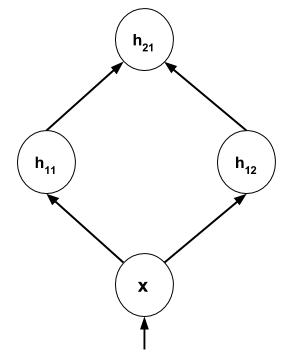
\includegraphics[scale=0.35]{sig2d}
          		  \end{center}
                  Plot the following functions: $h_{11}(x)$, $h_{12}(x)$ and $h_{21}(x)$ for $x \in (-1, 1)$
                  \begin{solution}
                  		\begin{center}
                  			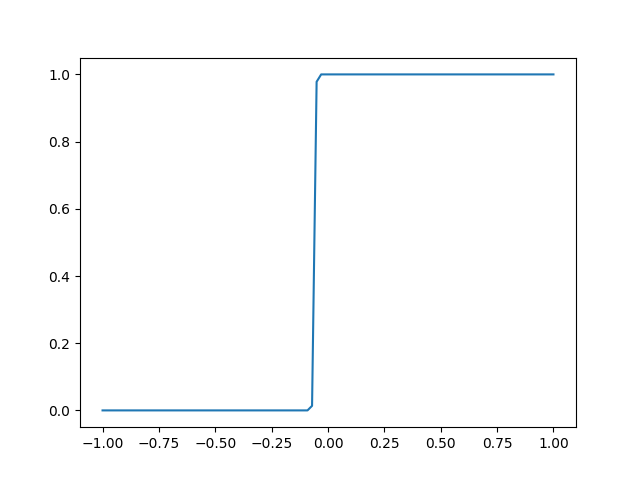
\includegraphics[scale=0.8]{h11}
                  			\captionof{figure}{$h11(x_1, x_2)$}
                  			\label{fig:h1}
                  		\end{center}
                  		
                  		\begin{center}
                  			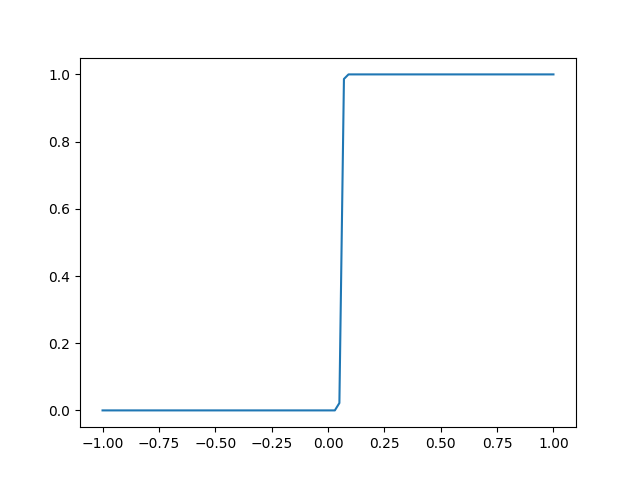
\includegraphics[scale=0.8]{h12}
                  			\captionof{figure}{$h12(x_1, x_2)$}
                  			\label{fig:h2}
                  		\end{center}
                  		
                  		\begin{center}
                  			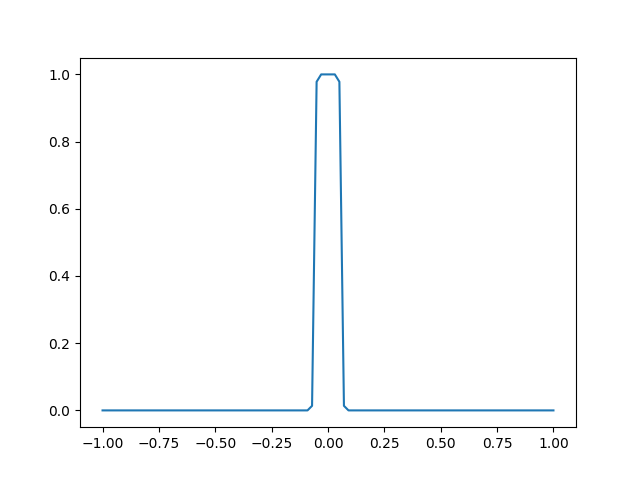
\includegraphics[scale=0.8]{h21}
                  			\captionof{figure}{$h21(x_1, x_2)$}
                  			\label{fig:h3}
                  		\end{center}
                  \end{solution}
            \part Now consider the variables $x_1, x_2$ and the functions $h_{11}(x_1, x_2), h_{12}(x_1, x_2), h_{13}(x_1, x_2), h_{14}(x_1, x_2)$, $h_{21}(x_1, x_2), h_{22}(x_1, x_2), h_{31}(x_1, x_2)$ and $f(x_1, x_2)$ such that   
   
                  \begin{align*}
                    h_{11}(x_1, x_2) &= \frac{1}{1 + e^{-(x_1 + 100x_2 + 200)}}  \\
                    h_{12}(x_1, x_2) &= \frac{1}{1 + e^{-(x_1 + 100x_2 - 200)}}  \\
                    h_{13}(x_1, x_2) &= \frac{1}{1 + e^{-(100x_1 + x_2 + 200)}}  \\
                    h_{14}(x_1, x_2) &= \frac{1}{1 + e^{-(100x_1 + x_2 - 200)}}  \\
                    h_{21}(x_1, x_2) &= h_{11}(x_1, x_2) - h_{12}(x_1, x_2)\\
                    h_{22}(x_1, x_2) &= h_{13}(x_1, x_2) - h_{14}(x_1, x_2)\\
                    h_{31}(x_1, x_2) &= h_{21}(x_1, x_2) + h_{22}(x_1, x_2)\\
                    f(x_1, x_2) &= \frac{1}{1 + e^{-(50h_{31}(x) - 100)}}  \\\\
                  \end{align*}
                  The above set of functions are summarized in the graph below.
                    \begin{center}
            		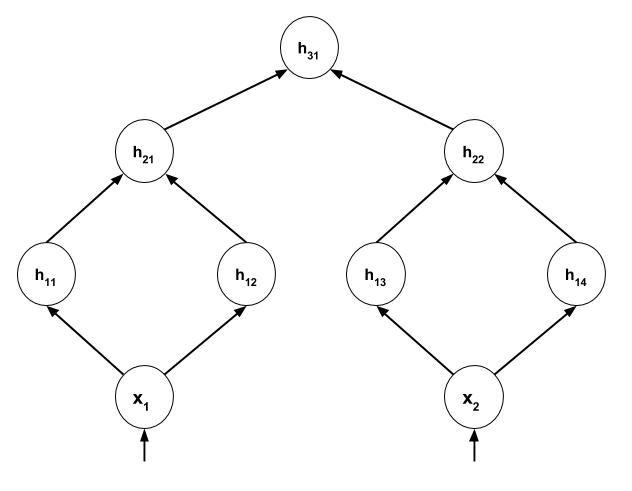
\includegraphics[scale=0.35]{sig3d}
          		  \end{center} 
                  Plot the following functions: $h_{11}(x_1, x_2), h_{12}(x_1, x_2), h_{13}(x_1, x_2), h_{14}(x_1, x_2), h_{21}(x_1, x_2),$ $h_{22}(x_1, x_2), h_{31}(x_1, x_2)$ and $f(x_1, x_2)$ for $x_1 \in (-5, 5)$ and $x_2 \in (-5, 5)$
                  \begin{solution}
                  		\begin{center}
                  			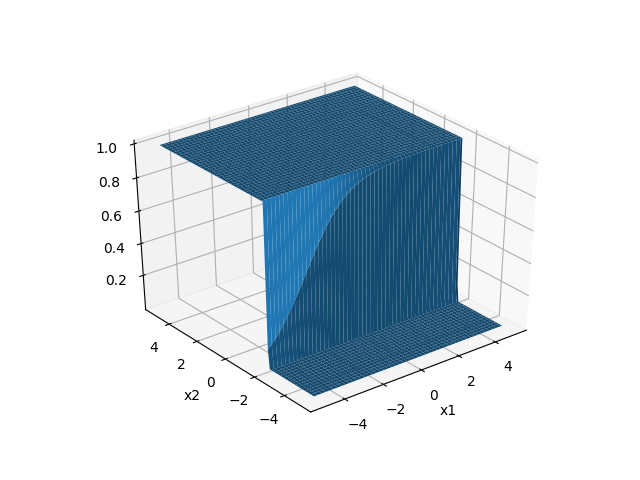
\includegraphics[scale=0.8]{h_11}
                  			\captionof{figure}{$h11(x_1, x_2)$}
                  			\label{fig:h11}
                  		\end{center}
                  		
                  		\begin{center}
                  			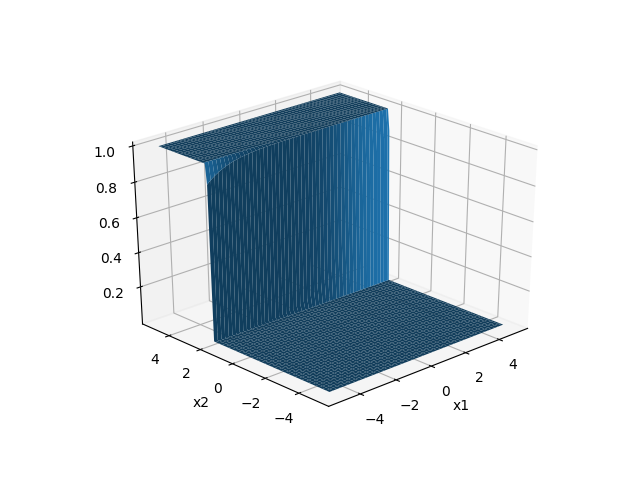
\includegraphics[scale=0.8]{h_12}
                  			\captionof{figure}{$h12(x_1, x_2)$}
                  			\label{fig:h12}
                  		\end{center}
                  		
                  		\begin{center}
                  			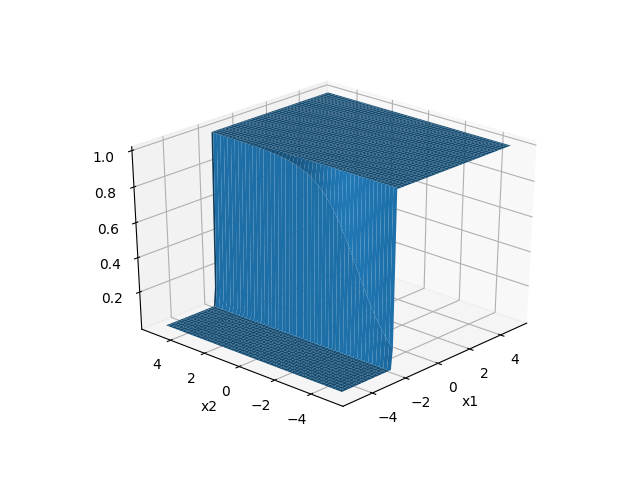
\includegraphics[scale=0.8]{h_13}
                  			\captionof{figure}{$h13(x_1, x_2)$}
                  			\label{fig:h13}
                  		\end{center}
                  		
                  		\begin{center}
                  			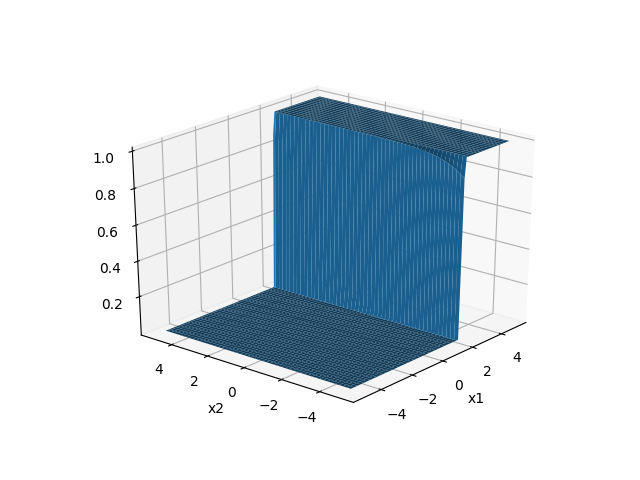
\includegraphics[scale=0.8]{h_14}
                  			\captionof{figure}{$h14(x_1, x_2)$}
                  			\label{fig:h14}
                  		\end{center}
                  		
                  		\begin{center}
                  			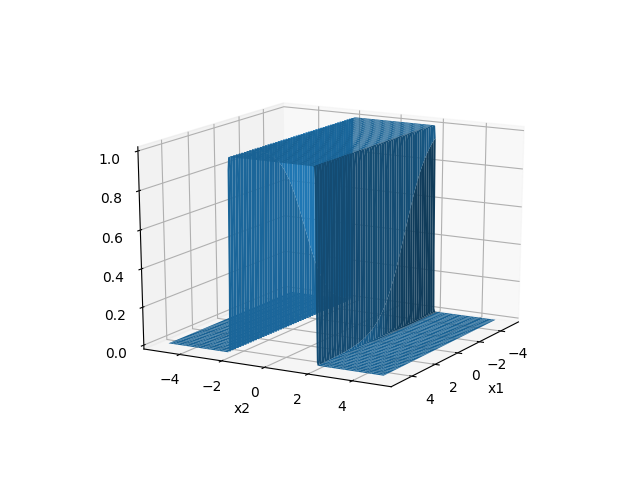
\includegraphics[scale=0.8]{h_21}
                  			\captionof{figure}{$h21(x_1, x_2)$}
                  			\label{fig:h21}
                  		\end{center}
                  		
                  		\begin{center}
                  			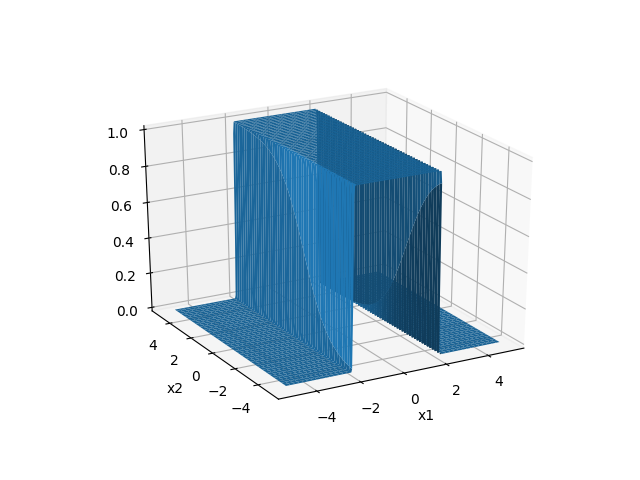
\includegraphics[scale=0.8]{h_22}
                  			\captionof{figure}{$h22(x_1, x_2)$}
                  			\label{fig:h22}
                  		\end{center}
                  		
                  		\begin{center}
                  			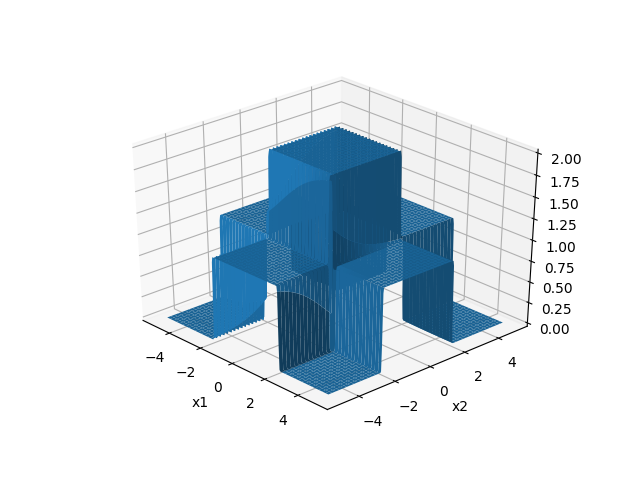
\includegraphics[scale=0.8]{h_31}
                  			\captionof{figure}{$h31(x_1, x_2)$}
                  			\label{fig:h31}
                  		\end{center}
                  		
                  		\begin{center}
                  			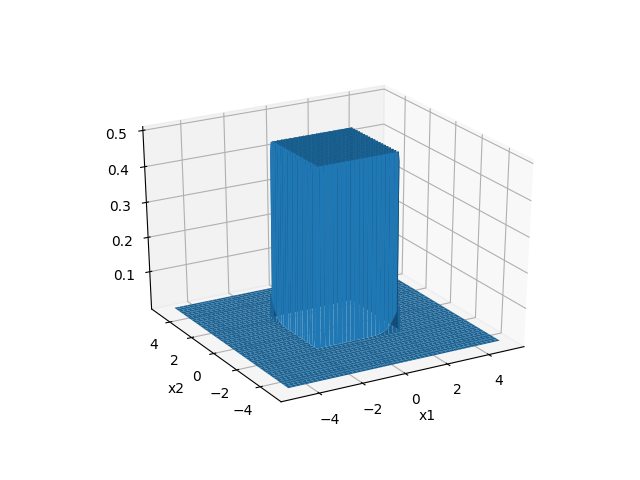
\includegraphics[scale=0.8]{f}
                  			\captionof{figure}{$f(x_1, x_2)$}
                  			\label{fig:f}
                  		\end{center}
                  \end{solution}
           \end{parts}
    

           
\end{questions}
\end{document} 